% Content for Collective Results subsection
% This file is included in the main conference paper via % Content for Collective Results subsection
% This file is included in the main conference paper via % Content for Collective Results subsection
% This file is included in the main conference paper via % Content for Collective Results subsection
% This file is included in the main conference paper via \input{CollectiveResults}
\begin{figure}
    \centering
    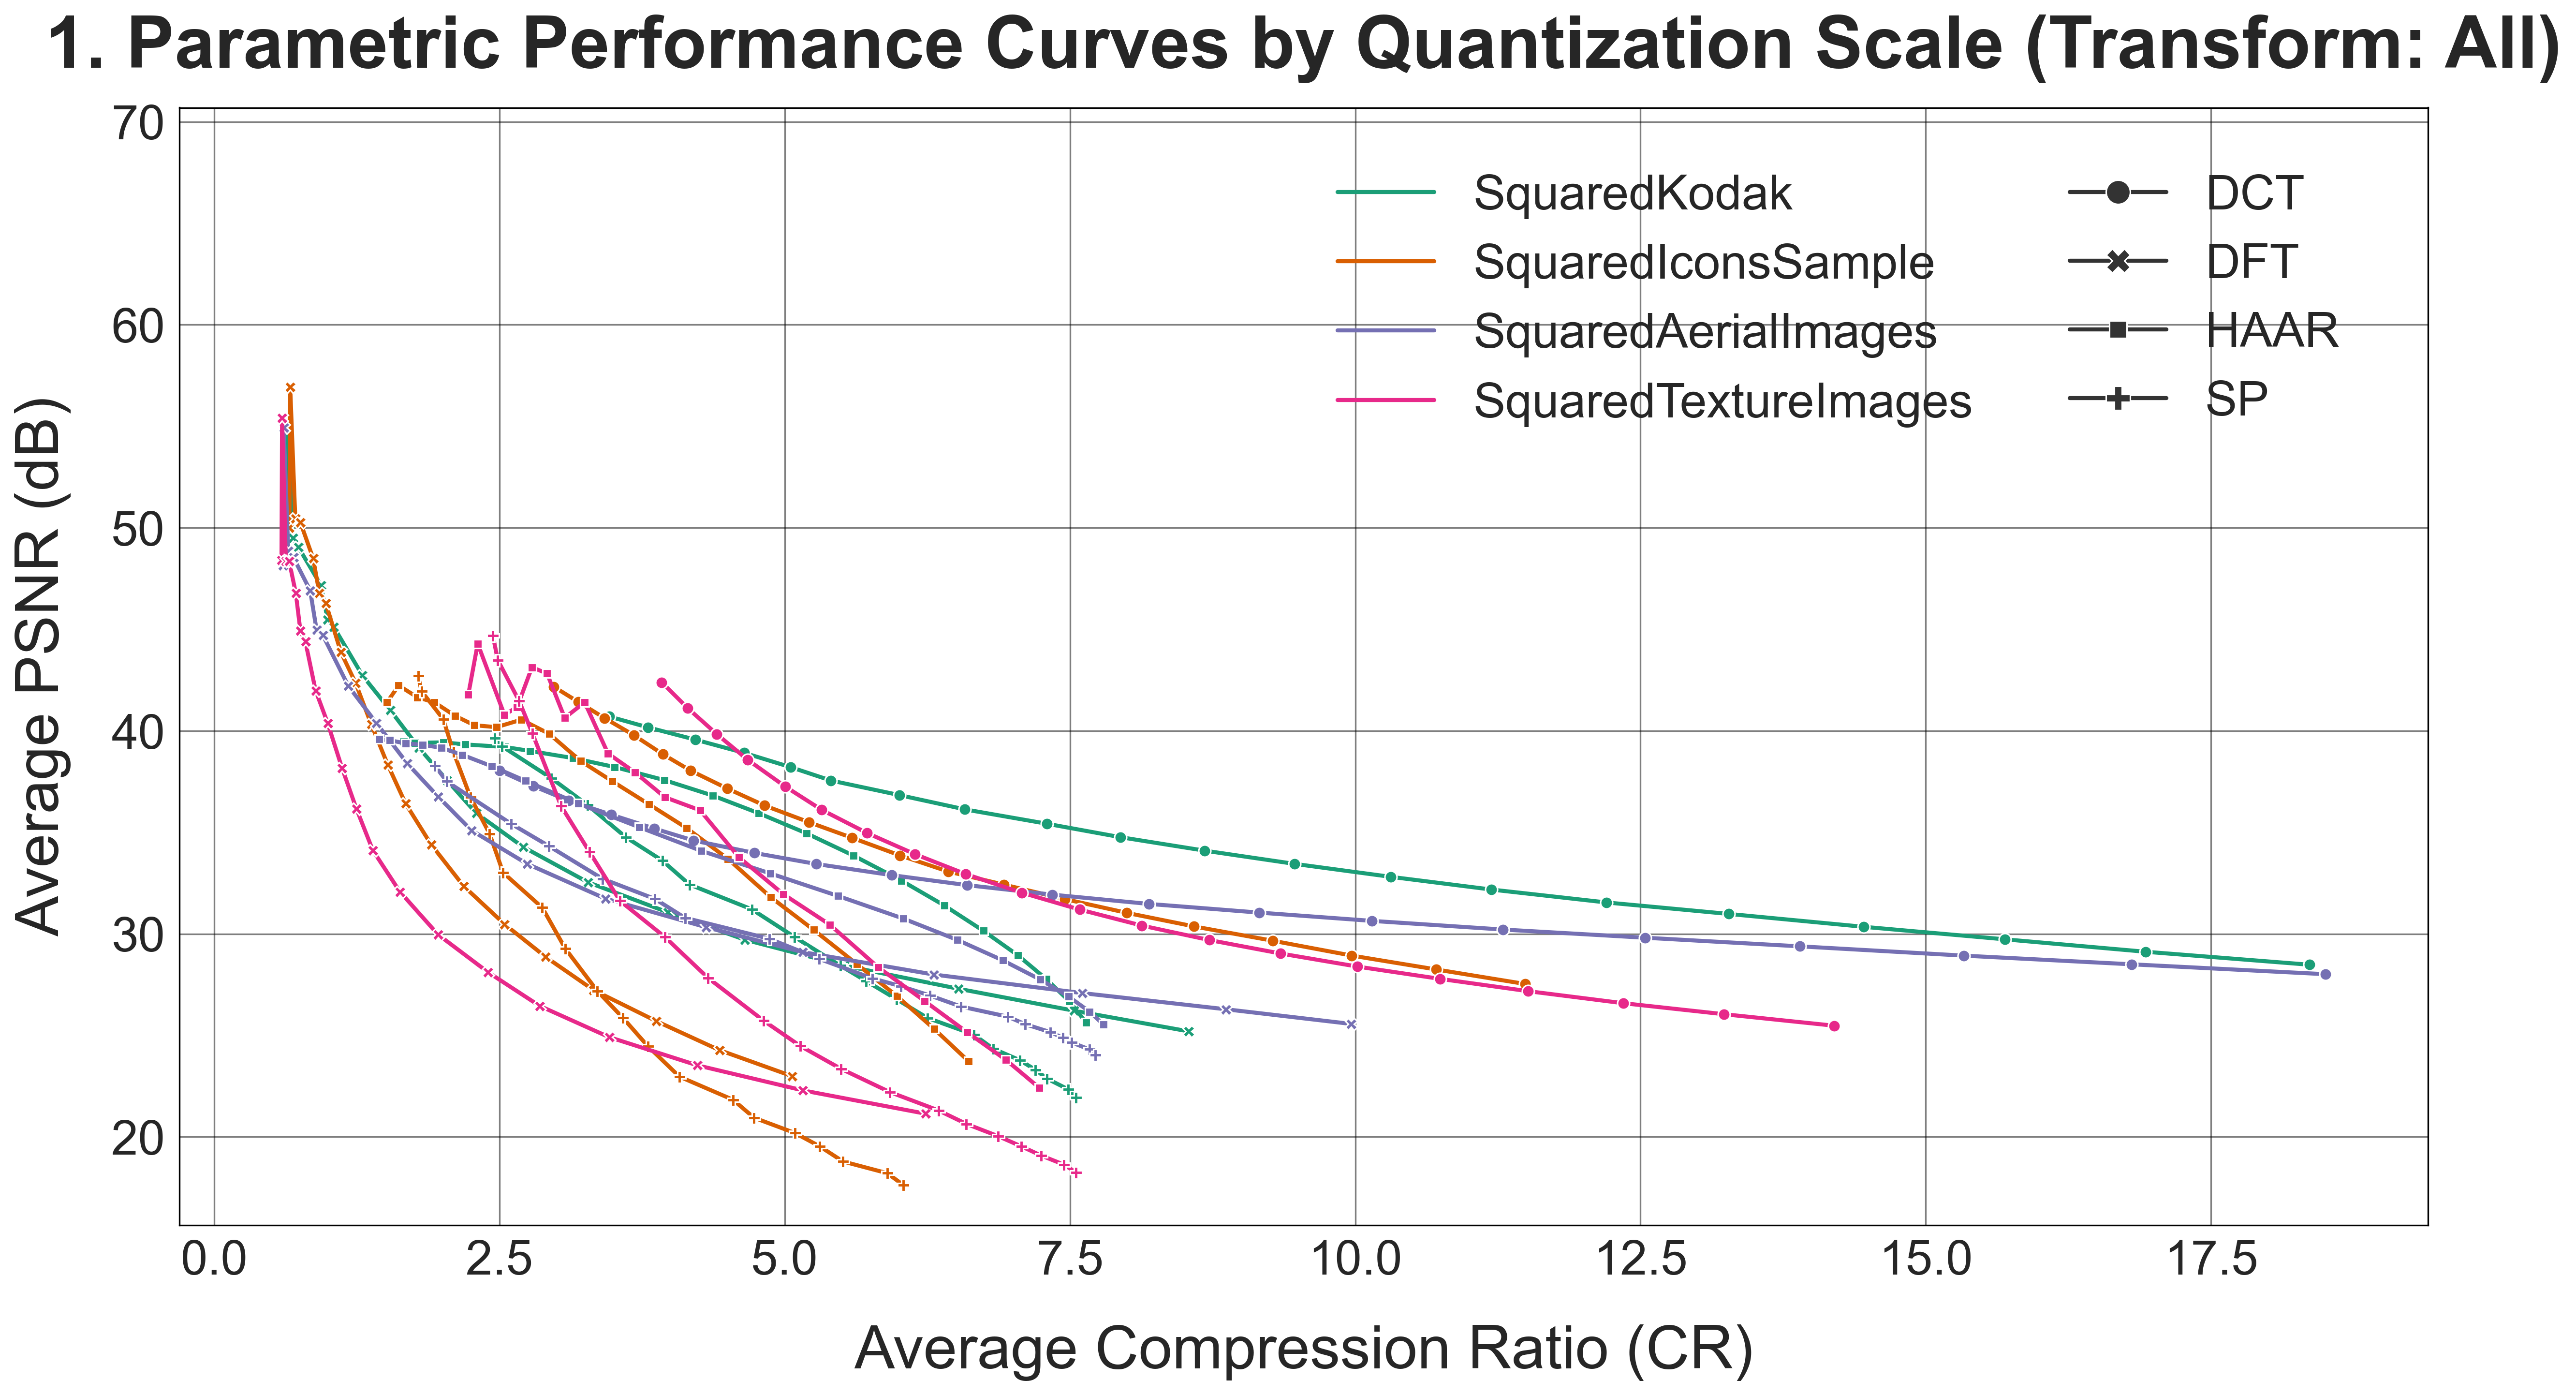
\includegraphics[width=1\linewidth]{results/plots/plot_1_parametric_curve_All.png}
    \caption{Compressed image similarity based on compression ratio by transform and dataset.}
    \label{fig:parametricAll}
\end{figure}

Firstly, as shown in fig. \ref{fig:parametricAll}, all transforms' had their quality of compressed images compared against compression ratio. Quality of compressed images, measured by the similarity between compressed and original image, or PSNR (db), is much higher for DCT, colored in blue, than all other transforms at all compression levels, with DCT additionally reaching higher compression levels than any other transform. Fig. \ref{fig:effectEntropyCoding} explores compression ratio by transform, with each box per transform representing compression ratio data with or without entropy coding used. For DCT and DFT, entropy coding generally increases compression ratio, with significant increases to the highest compression ratios achieved. On the other hand, Haar and SP see a flat decrease in compression ratio when entropy coding is used.

\begin{figure}
    \centering
    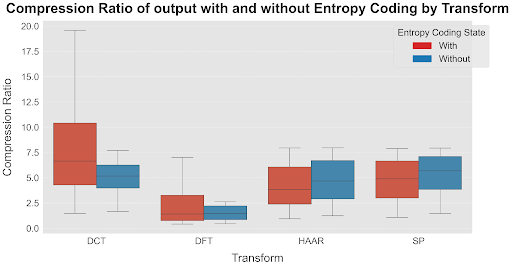
\includegraphics[width=1\linewidth]{results/plots/huffmancomparison.png}
    \caption{Effect of entropy encoding on compression ratio for all transforms}
    \label{fig:effectEntropyCoding}
\end{figure}


\begin{figure}
    \centering
    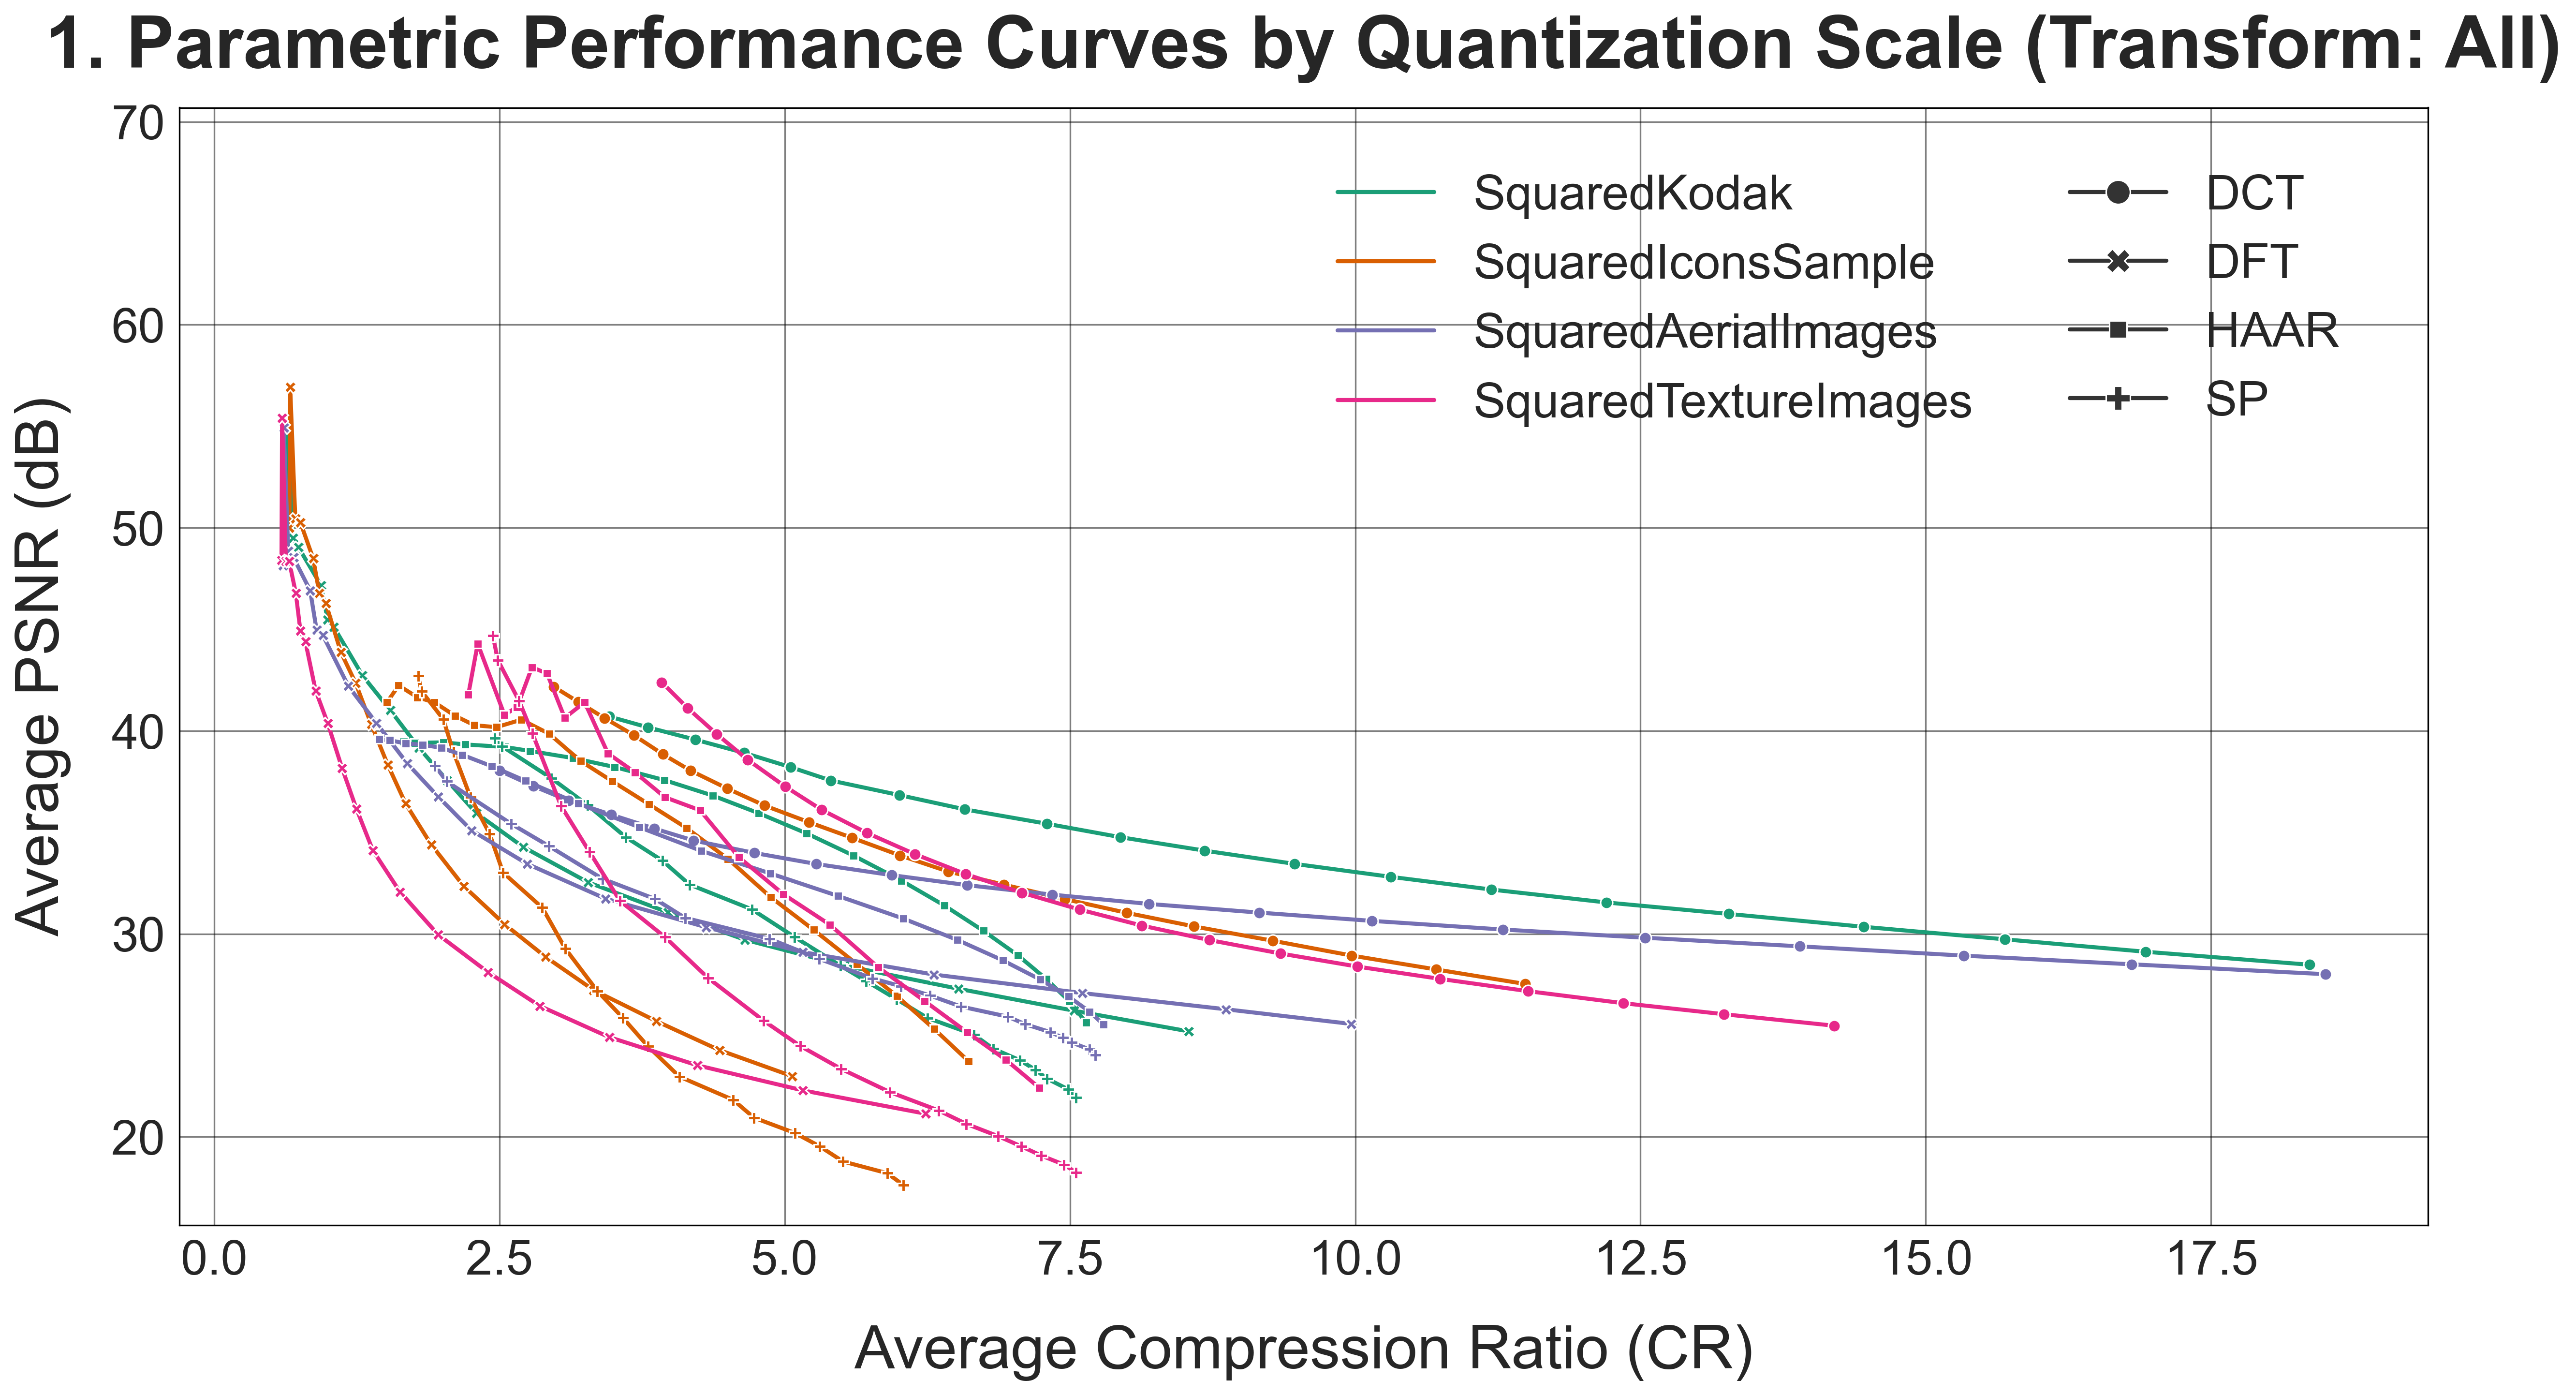
\includegraphics[width=1\linewidth]{results/plots/plot_1_parametric_curve_All.png}
    \caption{Compressed image similarity based on compression ratio by transform and dataset.}
    \label{fig:parametricAll}
\end{figure}

Firstly, as shown in fig. \ref{fig:parametricAll}, all transforms' had their quality of compressed images compared against compression ratio. Quality of compressed images, measured by the similarity between compressed and original image, or PSNR (db), is much higher for DCT, colored in blue, than all other transforms at all compression levels, with DCT additionally reaching higher compression levels than any other transform. Fig. \ref{fig:effectEntropyCoding} explores compression ratio by transform, with each box per transform representing compression ratio data with or without entropy coding used. For DCT and DFT, entropy coding generally increases compression ratio, with significant increases to the highest compression ratios achieved. On the other hand, Haar and SP see a flat decrease in compression ratio when entropy coding is used.

\begin{figure}
    \centering
    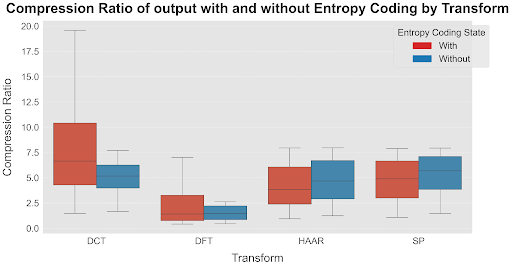
\includegraphics[width=1\linewidth]{results/plots/huffmancomparison.png}
    \caption{Effect of entropy encoding on compression ratio for all transforms}
    \label{fig:effectEntropyCoding}
\end{figure}


\begin{figure}
    \centering
    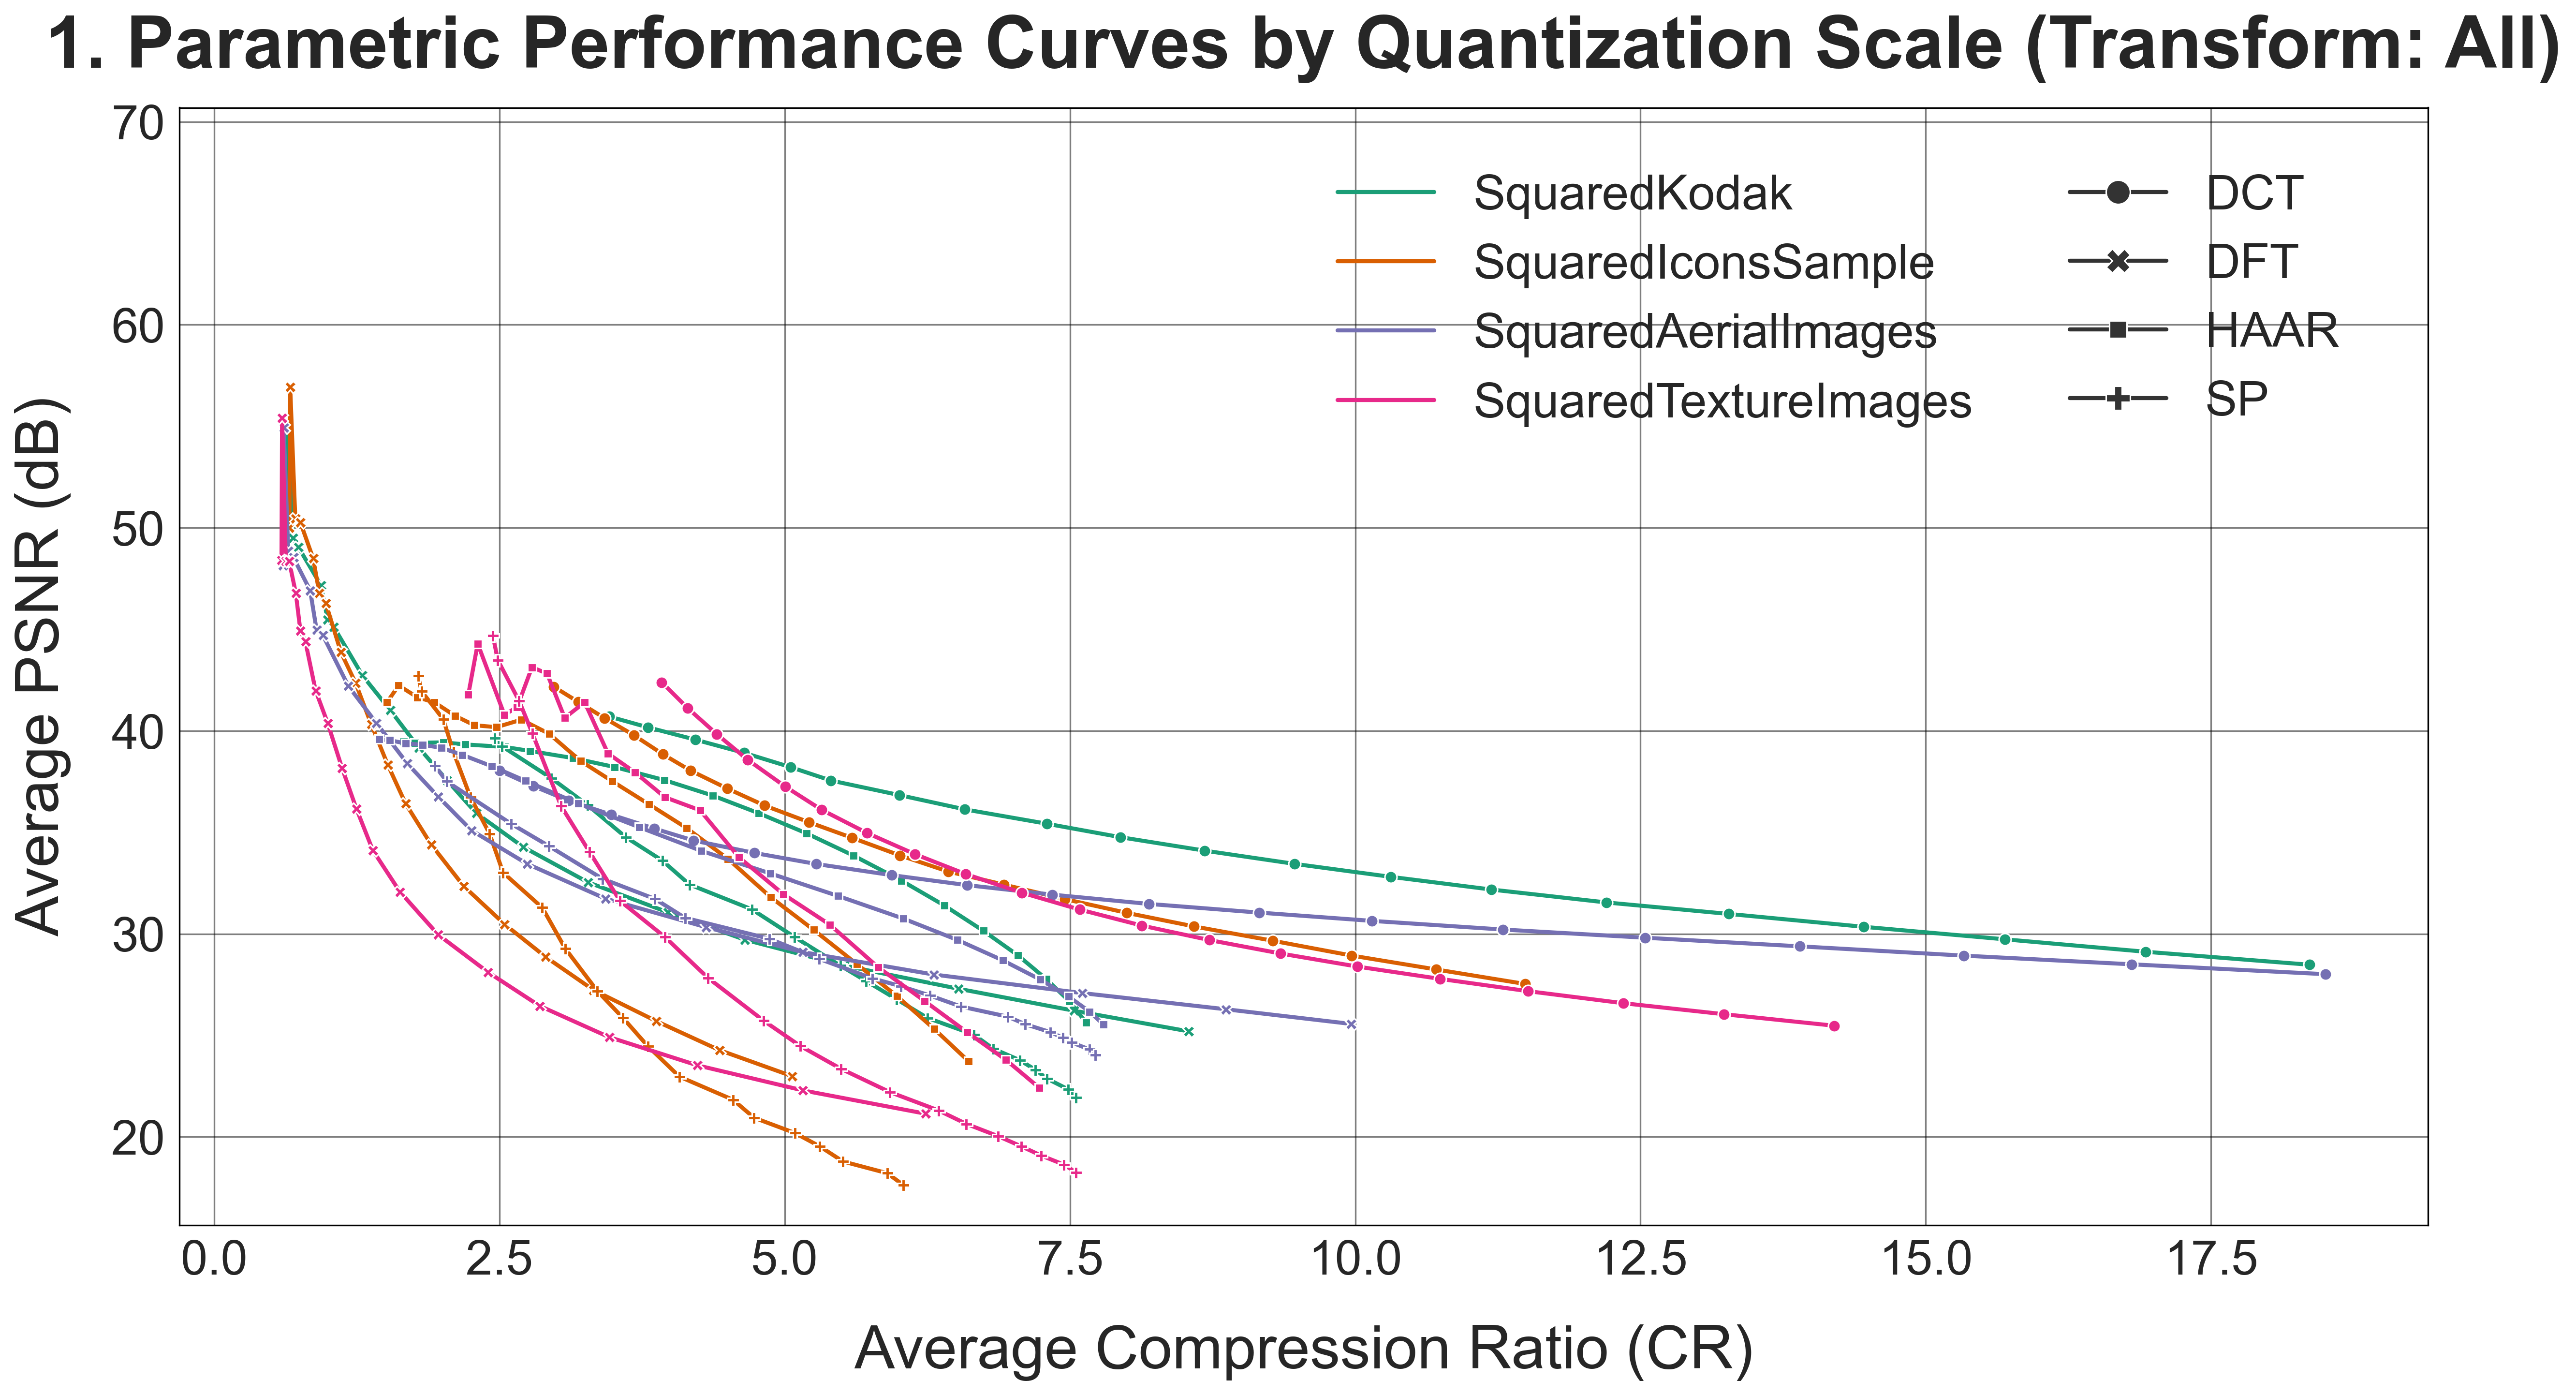
\includegraphics[width=1\linewidth]{results/plots/plot_1_parametric_curve_All.png}
    \caption{Compressed image similarity based on compression ratio by transform and dataset.}
    \label{fig:parametricAll}
\end{figure}

Firstly, as shown in fig. \ref{fig:parametricAll}, all transforms' had their quality of compressed images compared against compression ratio. Quality of compressed images, measured by the similarity between compressed and original image, or PSNR (db), is much higher for DCT, colored in blue, than all other transforms at all compression levels, with DCT additionally reaching higher compression levels than any other transform. Fig. \ref{fig:effectEntropyCoding} explores compression ratio by transform, with each box per transform representing compression ratio data with or without entropy coding used. For DCT and DFT, entropy coding generally increases compression ratio, with significant increases to the highest compression ratios achieved. On the other hand, Haar and SP see a flat decrease in compression ratio when entropy coding is used.

\begin{figure}
    \centering
    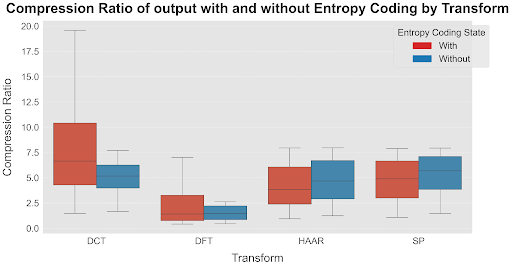
\includegraphics[width=1\linewidth]{results/plots/huffmancomparison.png}
    \caption{Effect of entropy encoding on compression ratio for all transforms}
    \label{fig:effectEntropyCoding}
\end{figure}


\begin{figure}
    \centering
    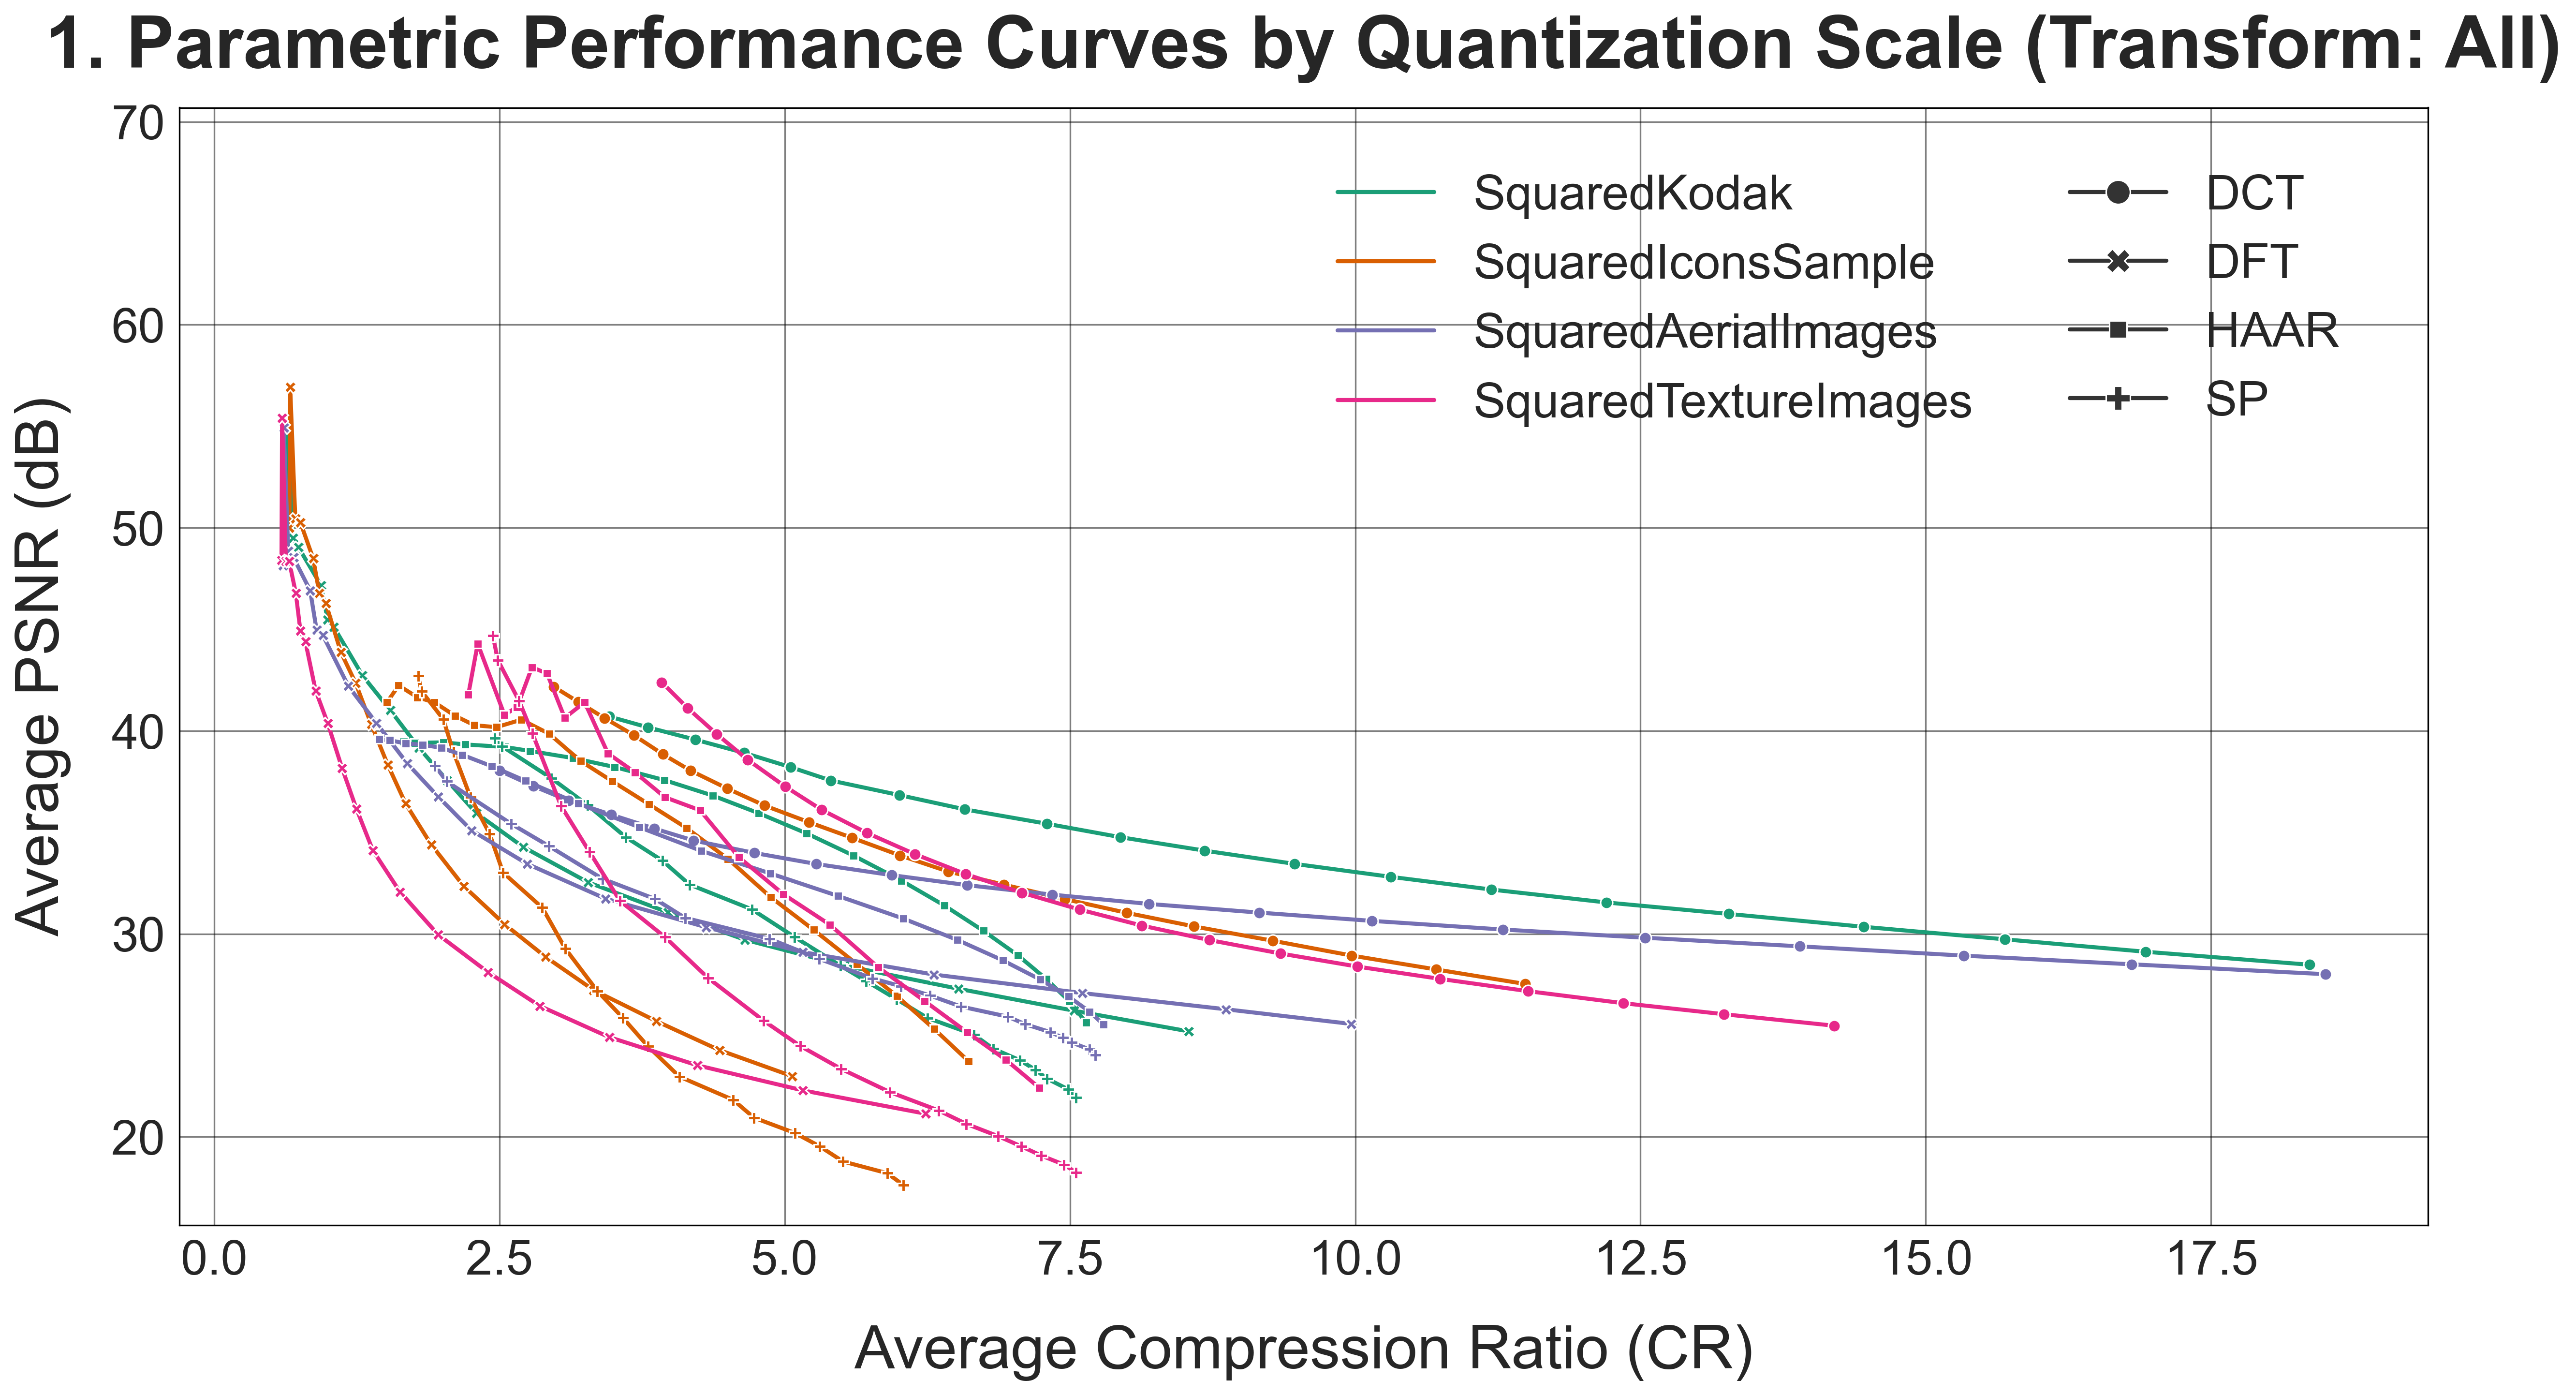
\includegraphics[width=1\linewidth]{results/plots/plot_1_parametric_curve_All.png}
    \caption{Compressed image similarity based on compression ratio by transform and dataset.}
    \label{fig:parametricAll}
\end{figure}

Firstly, as shown in fig. \ref{fig:parametricAll}, all transforms' had their quality of compressed images compared against compression ratio. Quality of compressed images, measured by the similarity between compressed and original image, or PSNR (db), is much higher for DCT, colored in blue, than all other transforms at all compression levels, with DCT additionally reaching higher compression levels than any other transform. Fig. \ref{fig:effectEntropyCoding} explores compression ratio by transform, with each box per transform representing compression ratio data with or without entropy coding used. For DCT and DFT, entropy coding generally increases compression ratio, with significant increases to the highest compression ratios achieved. On the other hand, Haar and SP see a flat decrease in compression ratio when entropy coding is used.

\begin{figure}
    \centering
    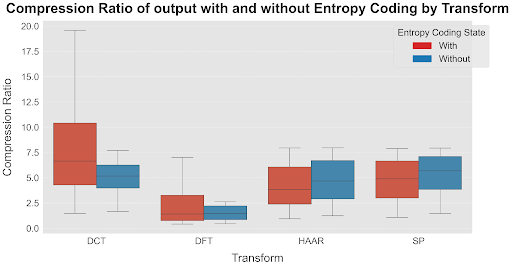
\includegraphics[width=1\linewidth]{results/plots/huffmancomparison.png}
    \caption{Effect of entropy encoding on compression ratio for all transforms}
    \label{fig:effectEntropyCoding}
\end{figure}

